\documentclass{beamer}
\usepackage[utf8]{inputenc}
\usepackage[T1]{fontenc}
\usepackage{lmodern}
\usepackage[scaled=.95]{libertine}
\usepackage{algorithm}
\usepackage{algorithmic}
\usepackage{subfigure}
%\usepackage{picins}%mix figures and text together
\usepackage{picinpar} 

%\usepackage[loosequotes]{MinionPro}
%\usepackage{MnSymbol}
%\pdfmapfile{+MinionPro.map}
\bibliographystyle{plain}
\usepackage[orientation=portrait,size=a0,scale=1.9]{beamerposter}

\usepackage{fixltx2e}
\usepackage{graphicx}
\usepackage{tabularx,multirow,booktabs}
\usepackage{relsize}
\setlength{\abovecaptionskip}{0pt}
\newcommand\LI[1]{\textrm{`#1'}}
\newcommand\acronym[1]{\textsmaller{\MakeUppercase{#1}}}

\usetheme{LLT-poster}
\usecolortheme{ComingClean}
\footimage{}%\includegraphics[width=.35\textwidth]{authors}}

\usepackage{tikz}

\title{An Efficient Online Event Detection Method for Microblogs via User Modeling}
\author[huangwaleking\string@gmail.com \hspace{.1em} \{pekingchenwei,tjwang\}@pku.edu.cn \hspace{.1em}citlmzhang@163.com]{Weijing \textsc{Huang} \and Wei \textsc{Chen} \and Lamei \textsc{Zhang} \and Tengjiao \textsc{Wang}}
\institute{\raisebox{-.2ex}{EECS, Peking University, Beijing}
\date{}
\begin{document}
\begin{frame}
\vskip-1ex
\begin{columns}[T]
\begin{column}{.46\textwidth}
\parbox[t][1200mm]{\textwidth}{
\begin{block}{Introduction}
\begin{itemize}
\item Detecting events in microblogs is important but still challenging.
        \begin{itemize}
                \item Tweet stream is a mixture of user interests and external events, it's difficult to distinguish them.
                \item Existing methods are ineffective since they ignore user interests or only model interests and events on a fixed dataset without scalability.
        \end{itemize}
\item We introduce an online learning model \textit{User Profile Based Interest and Event Topic Model} (UPIETM).
        \begin{itemize}
                \item exploiting user profile to discover events by filtering out user interest-related tweets;
                \item treating the arriving data as stream and run the detection in online learning style.
        \end{itemize}
\end{itemize}
\end{block}


\begin{block}{Relationship between Profile and Interests }
\begin{itemize}
        \item User profile is highly correlated to user's interests.
\end{itemize}
\begin{figure}[H]
        \centering
        \label{fig:profile} %% label for entire figure
        \subfigure[\tiny{user's profile on weibo}]{
                \label{fig:profile:a} %% label for first subfigure
                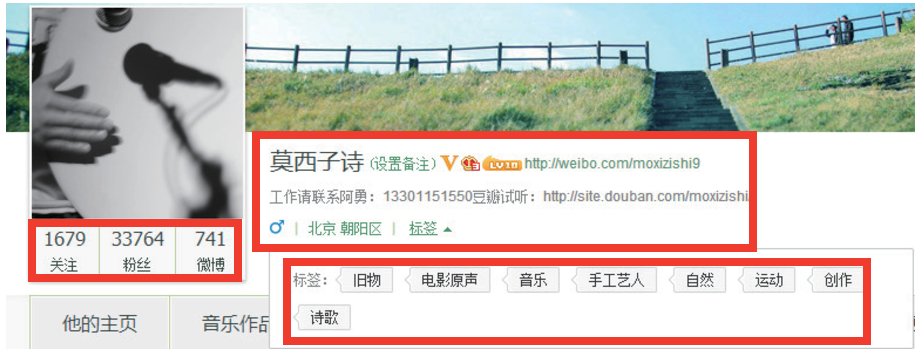
\includegraphics[height=3.5cm]{img/userProfile.pdf}
        }  
        \subfigure[\tiny{user's tweet on weibo}]{
                \label{fig:profile:b} %% label for second subfigure
                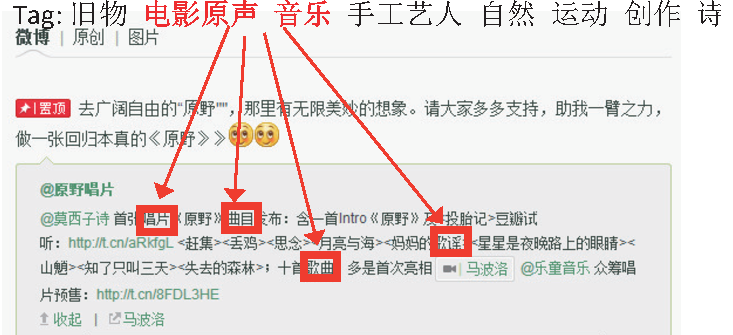
\includegraphics[height=3.5cm]{img/profileAndInterests.pdf}
        }
        \subfigure[\tiny{Andrew Ng}]{
                \label{fig:profile:c} %% label for first subfigure
                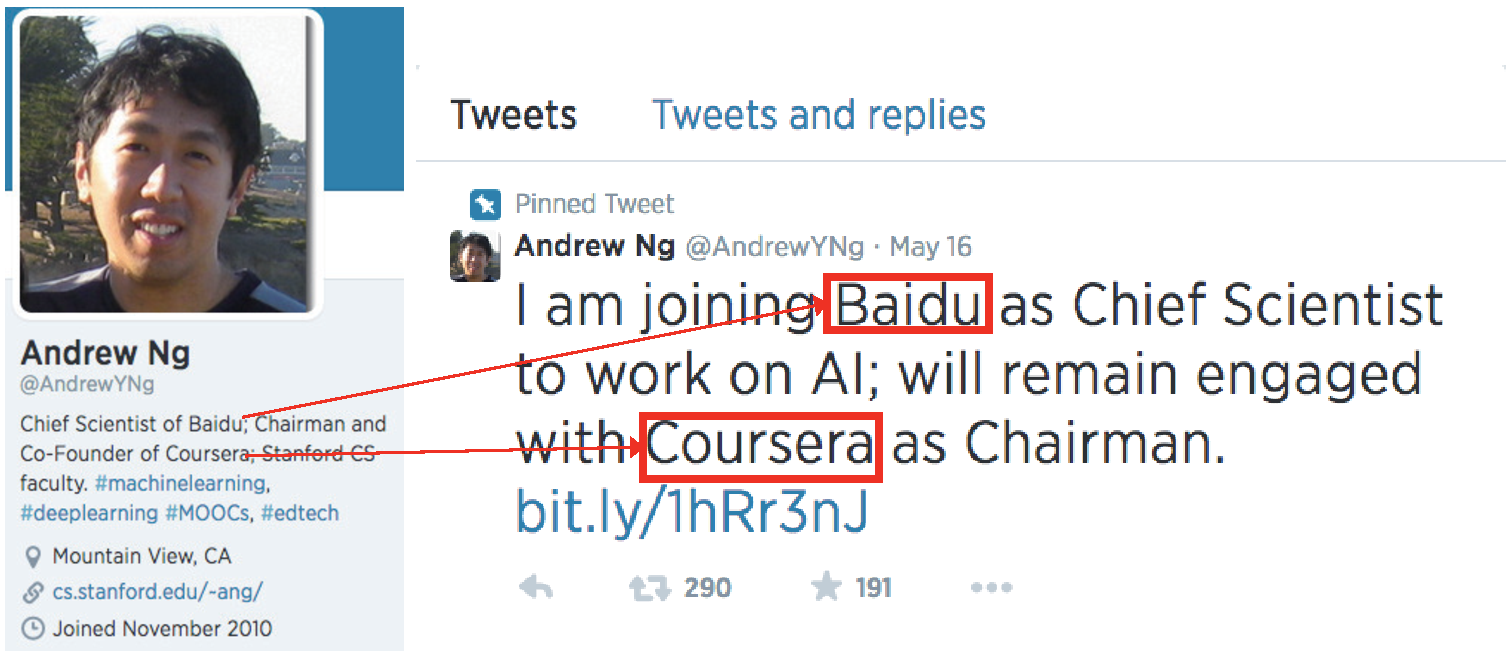
\includegraphics[height=3.5cm]{img/andrewNg.pdf}
        }  
        \subfigure[\tiny{Van Persie}]{
                \label{fig:profile:d} %% label for second subfigure
                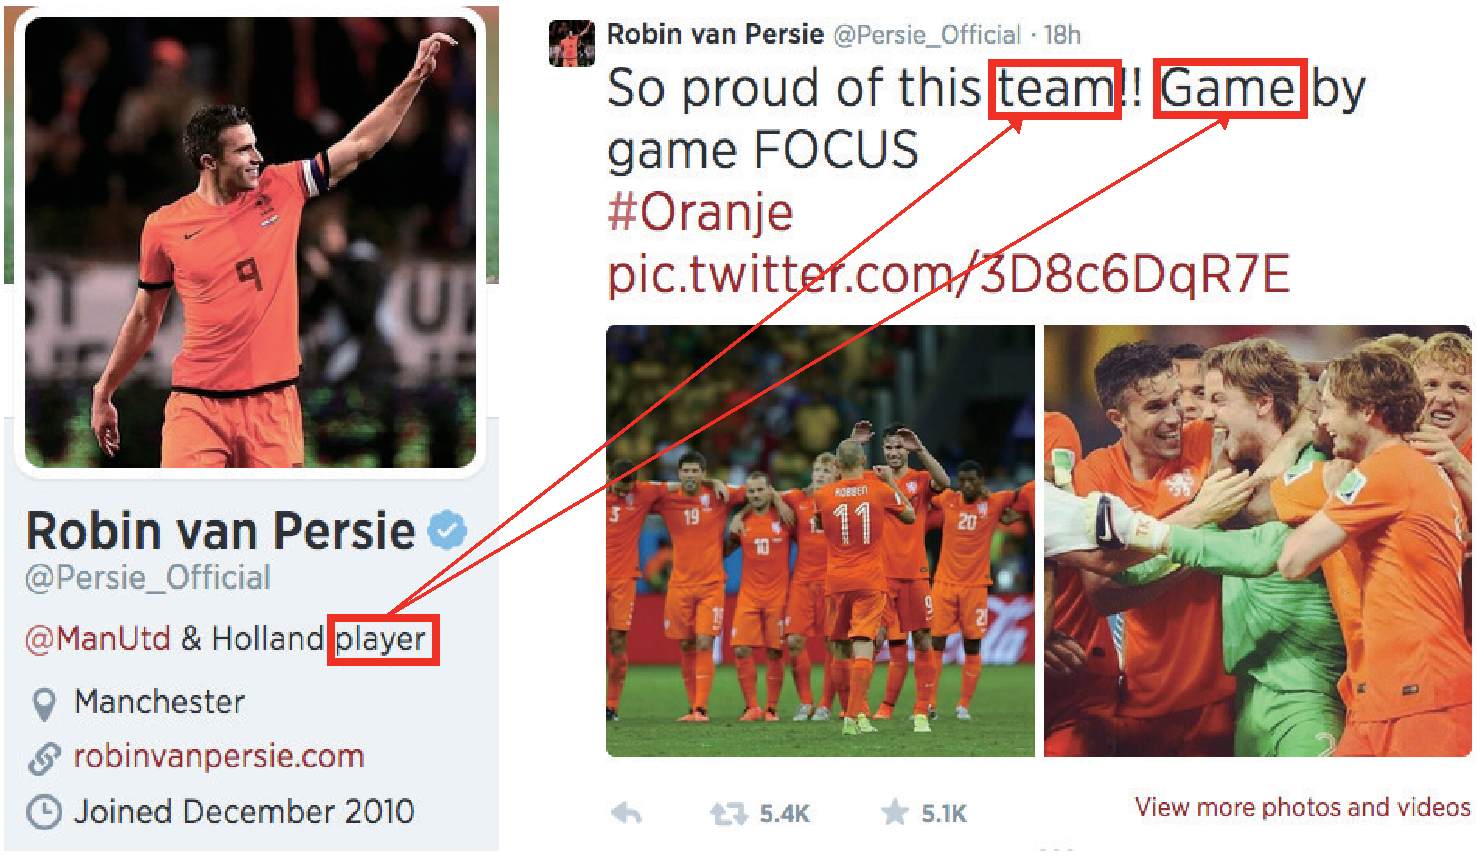
\includegraphics[height=3.5cm]{img/robinVanPersie.pdf}
        } 
        \caption{\small{Illustration of the relationship between user profile and user interests}} 
\end{figure}
\begin{itemize}
\item Users who have same user profiles also have similar interests.
        \begin{itemize}
                \item Word Clouds of \#DataMining and \#MachineLearning are more similar as there are 46.2\% \#MachineLearning users also choose \#DataMining tag.
        \end{itemize}
\end{itemize}
\begin{table}
\centering
\caption{\scriptsize{Word Clouds of tweets generated by users who have the specific user profile}}
\scalebox{1.0}{
\begin{tabular}{|l|c|c|c|c|c|c|}
        \hline
        \tiny{\#Buddhist} & \tiny{\#TOEFL} & \tiny{\#DataMinig} & \tiny{\#MachineLearning} & \tiny{\#PatternRecognization} & \tiny{\#Jewelry} & \tiny{\#Racing}\\
        \hline
        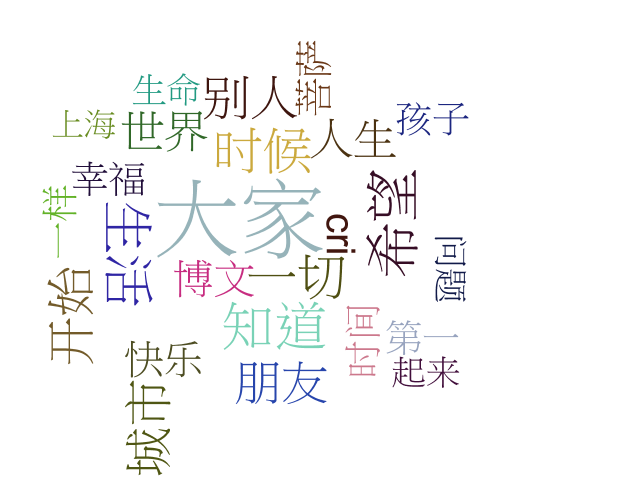
\includegraphics[width=.11\textwidth]{img/buddhist} & 
        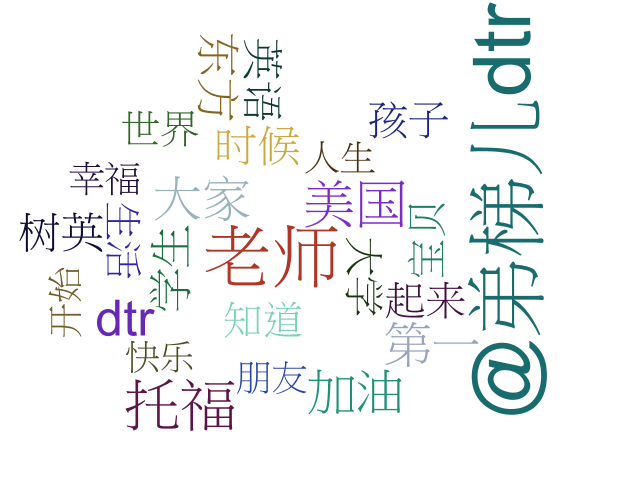
\includegraphics[width=.11\textwidth]{img/TOEFL} & 
        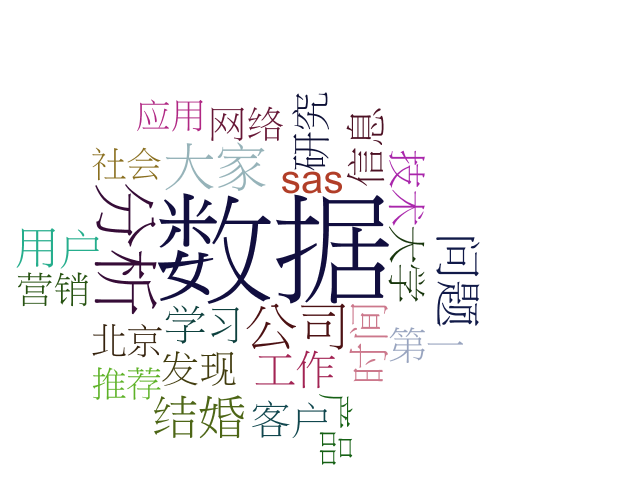
\includegraphics[width=.11\textwidth]{img/DataMining}&
        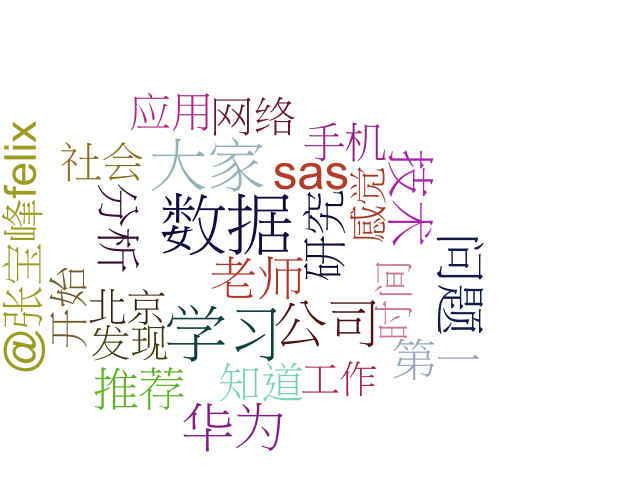
\includegraphics[width=.11\textwidth]{img/MachineLearning}&
        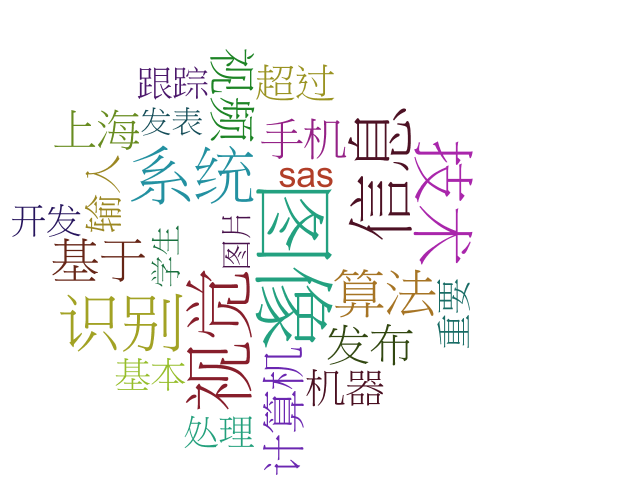
\includegraphics[width=.11\textwidth]{img/PatternRecognization}&
        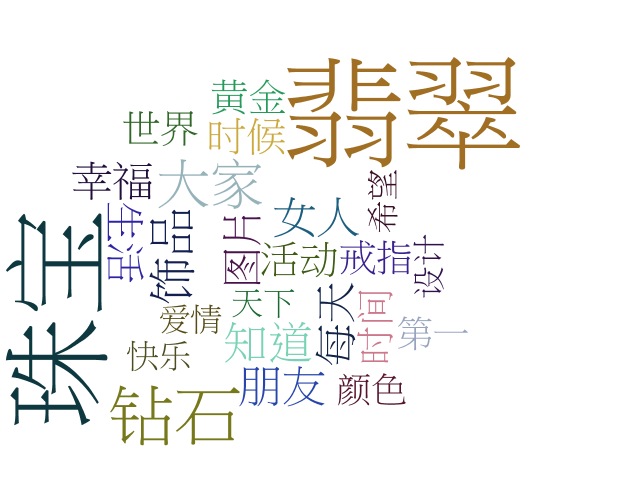
\includegraphics[width=.11\textwidth]{img/Jewelry}&
        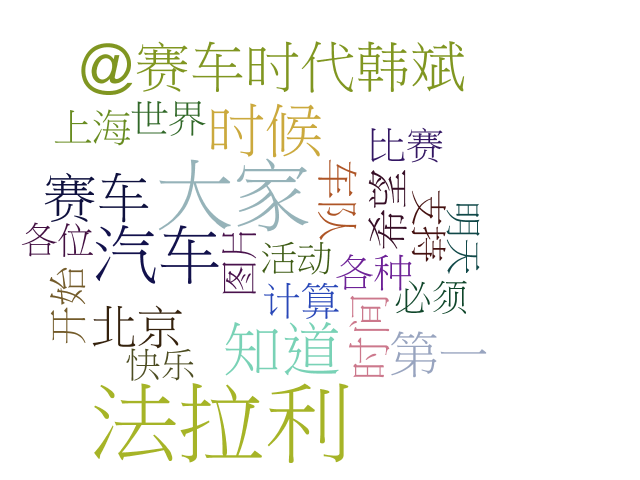
\includegraphics[width=.11\textwidth]{img/Racing}\\
        \hline
\end{tabular}
}
\end{table}     
\end{block}

\begin{block}{Proposed Model}
\begin{itemize}
\item User Profile Based Interest and Event Topic Model 
        \begin{itemize}
                \item main idea: user profiles are more stable to reflect user's interests than tweets; external events draw global attention in short time.
        \end{itemize}
\end{itemize}
\begin{columns}
        \begin{column}{.5\textwidth}
                \begin{itemize}
                        \item generative process
                        \begin{itemize}
                                \item \tiny{user generates hidden profile topic \(s_{un}\) from user-interest distribution \(\theta_u\), then generates profile token \(p_{un}\) from multinomial distribution \(\psi_{s_{un}}\).}
                                % \item user post interest-related tweets based on word-topic distribution \(\phi_k\), or event-related tweets from \(\varphi_{te}\).
                                \item \tiny{user decides to post interest-related tweet or event-related tweet according to switcher \(y_{ud}\).}
                                \item \tiny{if \(y_{ud}=0\), generates tweet's hidden topic \(z_{ud}\) from user's profile hidden topic \(\{s_{u1},\cdots,s_{un}\} \)uniformly, then generates tweet tokens from word-interest distribution \(\phi_{z_{ud}}\).}
                                \item \tiny{if \(y_{ud}=1\), generates tweet's hidden topic \(z_{ud}\) from event-timewindow distribution \(\eta_t\), then generates tweet tokens from word-event distribution \(\varphi_{t,z_{ud}}\).}
                        \end{itemize}
                \end{itemize}
        \end{column}
        \begin{column}{.5\textwidth}
                \begin{figure}
                        \centering
                        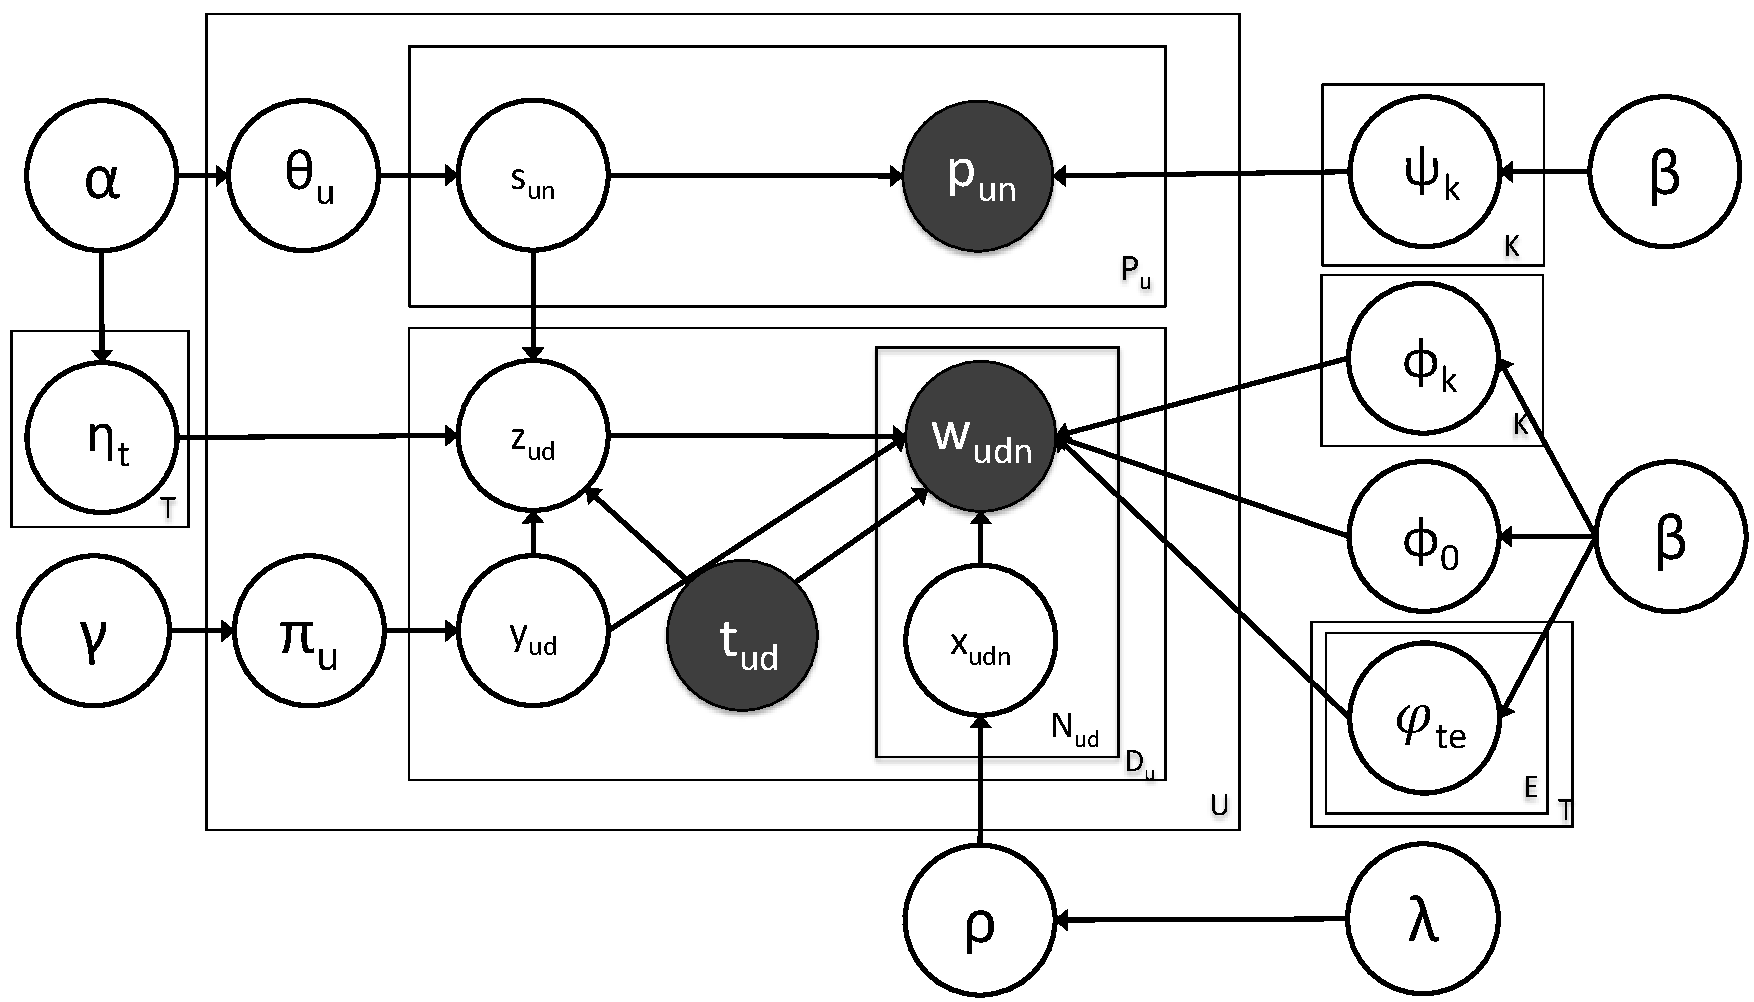
\includegraphics[height=10cm]{img/timeUserTagLDAIV.pdf}
                        \caption{Illustration of UPIETM}
                        \label{fig:Illustration of UPIETM}
                \end{figure} 
        \end{column}
\end{columns}

\end{block}

\begin{block}{Batch Learning}
\begin{itemize}
\item Gibbs Sampling
	\begin{itemize}
	\item 1st phase: sample user profile's hidden topic \(s_{un}\).
	\item 2nd phase: joint sample tweet's hidden topic \(z_{ud}\) and switcher \(y_{ud}\).
	\end{itemize}
\item Complexity: \(O(I_1 K|P|+I_2 K|W|+I_2 E|W|)\)
	\begin{itemize}
	\item \scriptsize{\(I_1\): iteration number of first phase sampling.}
	\item \scriptsize{\(I_2\): iteration number of second phase sampling.}
	\item \scriptsize{\(K\), \(E\): number of user interest related topics and number events in each time window.}
	\item \scriptsize{\(|P|\):  number of total user profile tokens.}
	\item \scriptsize{\(|W|\): number of total tweet tokens.}
	\end{itemize}
\end{itemize}
\end{block}
}
\end{column}

\begin{column}{.46\textwidth}
\parbox[t][1200mm]{\textwidth}{
\begin{block}{Online Learning}
\begin{itemize}
\item Batch Learning is expensive
\item Event detection should be processed in online style.
\item But how to deal with new words? 
        \begin{itemize}
                \item smoothing for new words
        \end{itemize}
\begin{figure}[H]
        \centering
        \label{fig:subfig} %% label for entire figure
        \subfigure[online processing]{
                \label{fig:subfig:a} %% label for first subfigure
                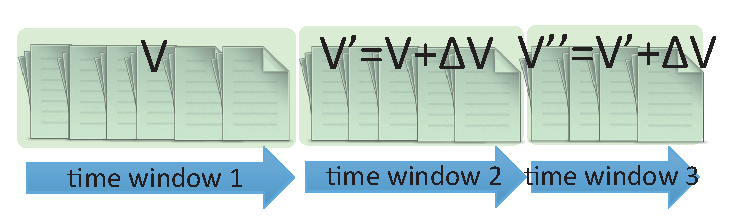
\includegraphics[height=4.3cm]{img/stream1.pdf}
        }  
        \subfigure[smoothing for new words]{
                \label{fig:subfig:b} %% label for second subfigure
                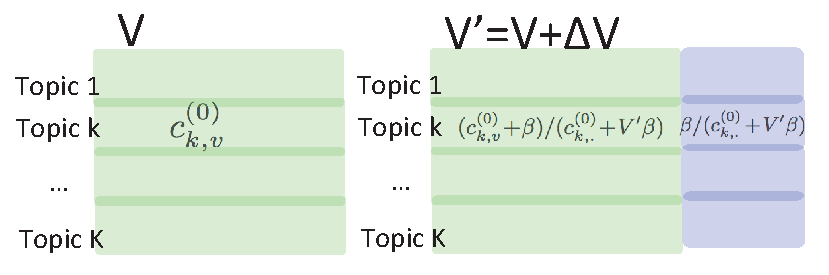
\includegraphics[height=4.3cm]{img/stream2.pdf}
        } \hspace{1in}
        \caption{\footnotesize{Illustration on how to reuse the word-topic distribution in online style}}
\end{figure}

\end{itemize}
\end{block}

\begin{block}{Weibo Dataset}
        \begin{columns}
                \begin{column}{.55\textwidth}
                        \begin{itemize}
                                \item \footnotesize{from Jan 2012 to Dec 2012}
                                \begin{itemize}
                                        \item \footnotesize{split dataset by week}
                                        \item \footnotesize{segment Chinese words}
                                        \item \footnotesize{remove stop words, low freqency words}
                                        \item \footnotesize{remove tweets whose token number is less than 3}
                                        \item \footnotesize{remove users who has less than 2 hashtags in profile}
                                \end{itemize}
                        \end{itemize}
                \end{column}
                \begin{column}{.45\textwidth}
                        \begin{table}
                                \centering
                                \caption{\scriptsize{statistics of processed dataset}}
                                \scalebox{0.44}{
                                        \begin{tabular}{|c|r|r|r|r|} \hline
                                         & \#user  & \#profile token & \#tweet & \#tweet token\\ \hline
                                         %\footnote{This dataset is available for reproducibility research. We have anonymized our name. http://...} 
                                        whole year& 252,369&  1,470,080 & 16,421,167 & 251,686,571\\ \hline
                                        week1 & 9,785 &  73,307& 31,503 & 440,217\\ \hline
                                        week2 & 29,721 & 222,280 & 242,554 & 3,679,979\\ \hline
                                        week3 & 30,891 & 231,042& 254,698 & 3,881,633\\ \hline
                                        week4 & 29,788 & 221,214& 237,456 & 3,510,934\\ \hline
                                        week5 & 24,256 & 179,292& 190,037 & 2,749,539\\ \hline
                                        \end{tabular}
                                }
                                \label{statisticsOfDataset}
                        \end{table}
                \end{column}
        \end{columns}

\end{block}

\begin{block}{Case Study}
\begin{figure}
\centering
        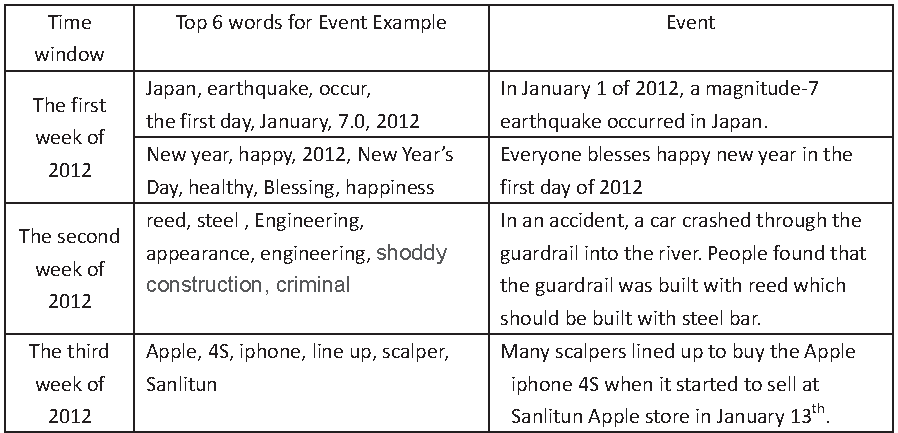
\includegraphics[width=.95\textwidth]{img/Event3.pdf}
        \caption{Events detected by UPIETM}
        \label{fig:event}
\end{figure}
\begin{itemize}
\item timeUserLDA\cite{timeUserLDA:2012} failed to discover the \emph{shoddy construction} event in the second week.
\end{itemize}
\end{block}

\begin{block}{Efficiency}
\begin{figure}[H]
        \centering
        \label{fig:subfig} %% label for entire figure
        \subfigure[the convergence of complete loglikelihood of UPIETM vs LDA]{
                \label{fig:subfig:a} %% label for first subfigure
                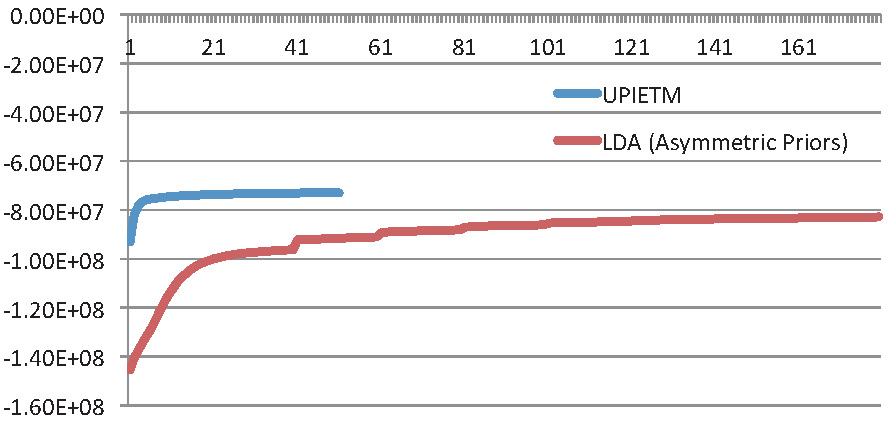
\includegraphics[height=8cm]{img/completeLoglikelihood.pdf}
        }  
        \subfigure[2nd]{
                \label{fig:subfig:b} %% label for second subfigure
                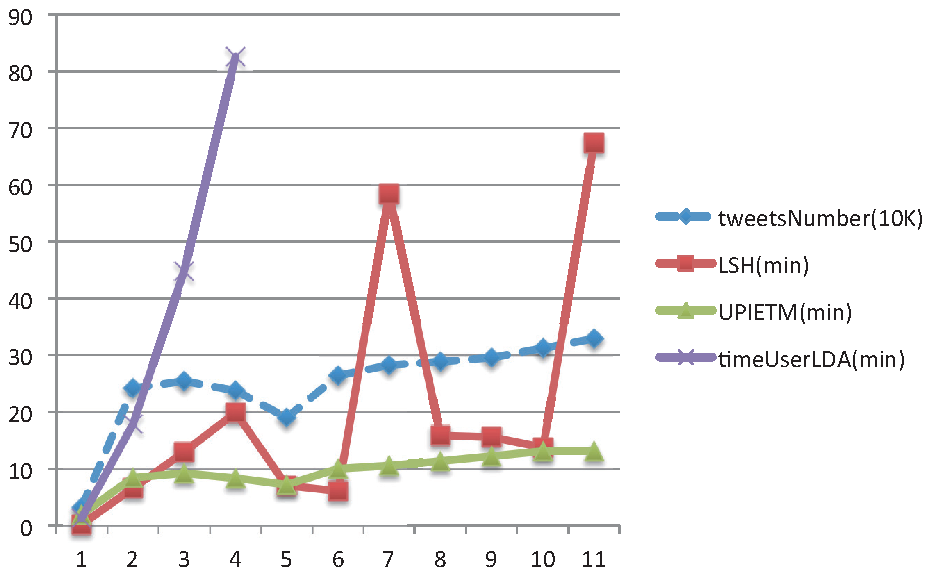
\includegraphics[height=8cm]{img/efficiencyCompareWithLSH.pdf}
        } \hspace{1in}
        \caption{Illustration on clustering result with different C} 
\end{figure}

\end{block}


%\begin{block}{Conclusion}
%\begin{itemize}
%\item Low thresholds ($\alpha,\beta$): more coverage; low precision %(false positives)
%\end{itemize}
%\end{block}


\begin{block}{References}
\setbeamertemplate{bibliography entry author}{\vspace*{-1.25ex}\raggedright}
\setbeamercolor{bibliography entry author}{fg=black}
\setbeamerfont{bibliography entry author}{size=\small}
\setbeamertemplate{bibliography item}[text]
\begin{thebibliography}{9}
\bibitem{timeUserLDA:2012}
\footnotesize{Qiming Diao, Jing Jiang, Feida Zhu, and Ee-Peng Lim. Finding bursty topics from microblogs. In: \emph{ACL 2012}.}
\bibitem{LSH:2010}
\footnotesize{Streaming first story detection with application to twitter. In: \emph{HLT-NAACL 2010}.}
\end{thebibliography}
\vspace*{-1.25ex}
\end{block}
}
\end{column}

\end{columns}
\end{frame}
\end{document}
